\chapter{Introduction}
Total Knee Arthroplasty (TKA) is a standard procedure for alleviating symptoms related to osteoarthritis in the knee. In 2018, orthopaedic surgeons performed more than 715,000 TKA operations in the United States \cite{agencyforhealthcareresearchandqualityHCUPFastStats}. This number is projected to increase to 3.48 million by 2030 \cite{kurtzProjectionsPrimaryRevision2007} due to an aging population and increased obesity rates. While TKA largely relieves symptomatic osteoarthritis, roughly 20\% of TKA patients express postoperative dissatisfaction, citing mechanical limitations, pain, and instability as the leading causes \cite{bakerRolePainFunction2007,bournePatientSatisfactionTotal2010,scottPredictingDissatisfactionFollowing2010}. Standard methods of musculoskeletal diagnosis cannot quantify the dynamic state of the joint, either pre- or post-operatively; clinicians must rely on static imaging (radiography, MRI, CT) or qualitative mechanical tests to determine the condition of the affected joint, and these tests cannot easily be performed during weight-bearing or dynamic movement when most pain symptoms occur. Unfortunately, most of the tools used to quantify 3D dynamic motion are substantially affected by soft-tissue artifacts \cite{gaoInvestigationSoftTissue2008,stagniQuantificationSoftTissue2005,linEffectsSoftTissue2016}, are prohibitively time-consuming or expensive \cite{daemsValidationThreedimensionalTotal2016}, or cannot be performed with equipment available at most hospitals.

Model-image registration is a process where a 3D model is aligned to match an object’s projection in an image \cite{brownSurveyImageRegistration1992}. Researchers have performed model-image registration using single-plane fluoroscopic or flat-panel imaging since the 1990s. Early methods used pre-computed distance maps \cite{lavalleeRecoveringPositionOrientation1995,zuffiModelbasedMethodReconstruction1999}, or shape libraries \cite{banksAccurateMeasurementThreedimensional1996,wallaceAnalysisThreedimensionalMovement1980,wallaceEfficientThreedimensionalAircraft1980} to match the projection of a 3D implant model to its projection in a radiographic image. With increasing computational capabilities, methods that iteratively compared implant projections to images were possible \cite{mahfouzRobustMethodRegistration2003,floodAutomatedRegistration3D2018,loweFittingParameterizedThreedimensional1991}. Most model-image registration methods provide sufficient accuracy for clinical joint assessment applications, including natural and replaced knees \cite{banksVivoKinematicsCruciateretaining1997,banks2003HapPaul2004,komistekVivoFluoroscopicAnalysis2003,burtonAutomaticTrackingHealthy2021}, natural and replaced shoulders \cite{kijimaVivo3dimensionalAnalysis2015,mahfouzVivoDeterminationDynamics,matsukiVivo3dimensionalAnalysis2011,sugiComparingVivoThreedimensional2021}, and extremities \cite{cenniKinematicsThreeComponents2012,cenniFunctionalPerformanceTotal2013,deaslaSixDOFVivo2006}. One of the main benefits of this single-plane approach is that suitable images can be acquired with equipment found in most hospitals. The main impediment to implementing this approach into a standard clinical workflow is the time and expense of human operators to supervise the model-image registration process. These methods require either (1) an initial pose estimate \cite{floodAutomatedRegistration3D2018,loweFittingParameterizedThreedimensional1991}, (2) a pre-segmented contour of the implant in the image \cite{brownSurveyImageRegistration1992,lavalleeRecoveringPositionOrientation1995}, or (3) a human operator to assist the optimization routine out of local minima \cite{mahfouzRobustMethodRegistration2003}. Each of these requirements makes model-image registration methods impractical for clinical use. Even state-of-the-art model-image registration techniques \cite{floodAutomatedRegistration3D2018} require human initialization or segmentation to perform adequately.

Machine learning algorithms automate the process of analytical model building, utilizing specific algorithms to fit a series of inputs to their respective outputs. Neural networks are a subset of machine learning algorithms that utilize artificial neurons inspired by the human brain’s connections \cite{marrEarlyProcessingVisual1976}. These networks have shown a great deal of success in many computer vision tasks, such as segmentation \cite{chanHistoSegNetSemanticSegmentation2019,wangDeepHighResolutionRepresentation2020,ronnebergerUNetConvolutionalNetworks2015}, pose estimation \cite{wuDeepGraphPose2020,kendallGeometricLossFunctions2017}, and classification \cite{krizhevskyImageNetClassificationDeep2017,qiPointNetDeepHierarchical2017,qiPointNetDeepLearning2017}. These capabilities might remove the need for human supervision from TKA model-image registration. Therefore, we propose a three-stage data analysis pipeline where a convolutional neural network (CNN) is used to segment, or identify, the pixels belonging to either a femoral or tibial component. Then, an initial pose estimate is generated comparing the segmented implant contour to a pre-computed shape library. Lastly, the initial pose estimate serves as the starting point for a Lipschitzian optimizer that aligns the contours of a 3D implant model to the contour of the CNN-segmented image.

\section{Background}
\subsection{Current Ortho Exams}
\input{src/1-Intro/1-1_background/ortho-exams.tex}
\subsection{Fluoroscopy}
\input{src/1-Intro/1-1_background/fluoroscopy.tex}
\subsection{Kinematics from Fluoroscopy}
\input{src/1-Intro/1-1_background/kinematics-from-fluoro.tex}

\section{Model-Image Registration}
\subsection{Geometric Transformations}
We start off with a brief overview of different 2D and 3D geometric primitives and transformations and how these can be represented computationally and mathematically.

\subsubsection{2D and 3D Points}
A point in N-dimensional space is represented as a set of N scalers, each representing a magnitude in that canonical direction (Eq. \ref{eq:point}).

\begin{equation}
    \mathbf{x} = \begin{bmatrix}
        x_1 \\ x_2 \\ \vdots \\ x_{N-1} \\ x_N
    \end{bmatrix} \in \mathbb{R}^N
    \label{eq:point}
\end{equation}

A pixel on an image is represented as a 2D point, $\mathbf{x} = [x , y]^{T}$, and a point in space is represented as a 3D point, $\mathbf{x} = [x , y , z]^{T}$. We can also represent these points using \emph{homogeneous coordinates} by adding a scale factor, $\tilde{w}$ (Eq. \ref{eq:homog-point}). Homogeneous points are equivalent up to a scale factor. For most model-image registration, $\tilde{w} = 1$, allowing us to perform rotations and translations simultaneously and successively with matrix multiplications.

\begin{equation}
    \tilde{\mathbf{x}} = \begin{bmatrix}
        \tilde{x_1} \\ \tilde{x_2} \\ \vdots \\ \tilde{x_N} \\ \tilde{w}
    \end{bmatrix} = \tilde{w}\begin{bmatrix}
        \mathbf{x}\\ 1
    \end{bmatrix} = \tilde{w}\bar{\mathbf{x}}
    \label{eq:homog-point}
\end{equation}

\subsubsection{2D Transformations}
The most basic transformation is a translation, which is simply adding two vectors together (Eq. \ref{eq:translation}).

\begin{equation}
    \begin{aligned}
        \mathbf{x'} &= \mathbf{x} + \begin{bmatrix}
            t_x \\ t_y
        \end{bmatrix} = \mathbf{x} + \mathbf{t}\\
        &\text{Or, using homogeneous coordinates and matrix multiplication} \\
        &= \begin{bmatrix}
            \mathbf{I} & \mathbf{t}
        \end{bmatrix}\bar{\mathbf{x}} \\
        &\text{Where $I$ is the $2 \times 2$ identity matrix}
    \end{aligned}
    \label{eq:translation}
\end{equation}

Next, we have a \emph{rotation transform}, which changes the orientation of the object, but not the shape (Eq. \ref{eq:2d-rot}, \ref{eq:2d-rot-mat}). 

\begin{equation}
    \begin{aligned}
        \mathbf{x}' = \mathbf{Rx}
    \end{aligned}
    \label{eq:2d-rot}
\end{equation}

where
\begin{equation}
    \mathbf{R} = \begin{bmatrix}
        cos\theta & -sin \theta \\ sin \theta & cos \theta 
    \end{bmatrix}
    \label{eq:2d-rot-mat}
\end{equation}

This will rotate an object $\theta$ in the counter clockwise direction. 

A translation and rotation can be performed together by replacing the $\mathbf{I}$ in Eq. \ref{eq:translation} with $\mathbf{R}$ from Eq. \ref{eq:2d-rot-mat}. (Eq. \ref{eq:2d-rot-trans}), this transformation preserves lengths and angles.
\begin{equation}
    \mathbf{x}' = \begin{bmatrix}
        \mathbf{R}_{2 \times 2} & \mathbf{t}
    \end{bmatrix} \bar{\mathbf{x}}
    \label{eq:2d-rot-trans}
\end{equation}


A scaled rotation will change the size of the object by some scaler factor, $s$ (Eq. \ref{eq:2d-scaled-rot}); this transformation preserves angles.

\begin{equation}
    \mathbf{x}' = \begin{bmatrix}
        s\mathbf{R}_{2 \times 2} & \mathbf{t}
    \end{bmatrix}\bar{\mathbf{x}}
    \label{eq:2d-scaled-rot}
\end{equation}

An affine transformation preserves parallelism, and is simply a pre-multiplication by an arbitrary $2 \times 3$ matrix (Eq. \ref{eq:2d-affine}).

\begin{equation}
    \begin{aligned}
        \mathbf{x}' &= \mathbf{A\bar{x}}\\
        &\text{where}\\
        \mathbf{A} &= \begin{bmatrix}
            a_{11} & a_{12} & a_{13} \\ a_{21} & a_{22} & a_{23}
        \end{bmatrix}
    \end{aligned}
    \label{eq:2d-affine}
\end{equation}
\subsection{Image Formation and Camera Properties}
Using our knowledge of geometric transformations and projective geometries, we can build up a model of a camera step by step. We standardize our reference frame by having the $z$ direction along the focal direction of the camera, the $x$ direction to the right, and the $y$ direction such that the right-hand rule is maintained. The origin is at the center of the camera.

We will describe the object of interest as a collection of points, $\mathbf{p} =  [x_i, y_i, z_i, 1] \text{ for } i = 1,2,\cdots,N$. For a complete picture, any given operation will be performed on all points. For simplicity, the following equations will demonstrate the process on a single point of the object.

First, we need to describe the location and orientation of the object with respect to the camera. This can be done with a 3D homogeneous transformation matrix (translation and rotation) (Eq. \ref{eq:4x4-homog-transformation}).

\begin{equation}
    \tilde{\mathbf{p}}' = \begin{bmatrix}
        R_{3 \times 3} & \mathbf{t}_{3 \times 1} \\ \mathbf{0}_{1 \times 3} & 1
    \end{bmatrix} \tilde{\mathbf{p}}
    \label{eq:4x4-homog-transformation}
\end{equation}

Then, we use a projective transformation that determines the perspective scaling between the objects actual location and the image place at the focal distance. Geometrically, this relationship can be visualized with similar triangles (Fig. \ref{fig:perspective-projection}), and quantified using the ratio of lengths (Eq. \ref{eq:perspective-projection}). In these equations, $f'$ is the focal distance in units of length.

\begin{figure}[h!]
    \begin{center}
        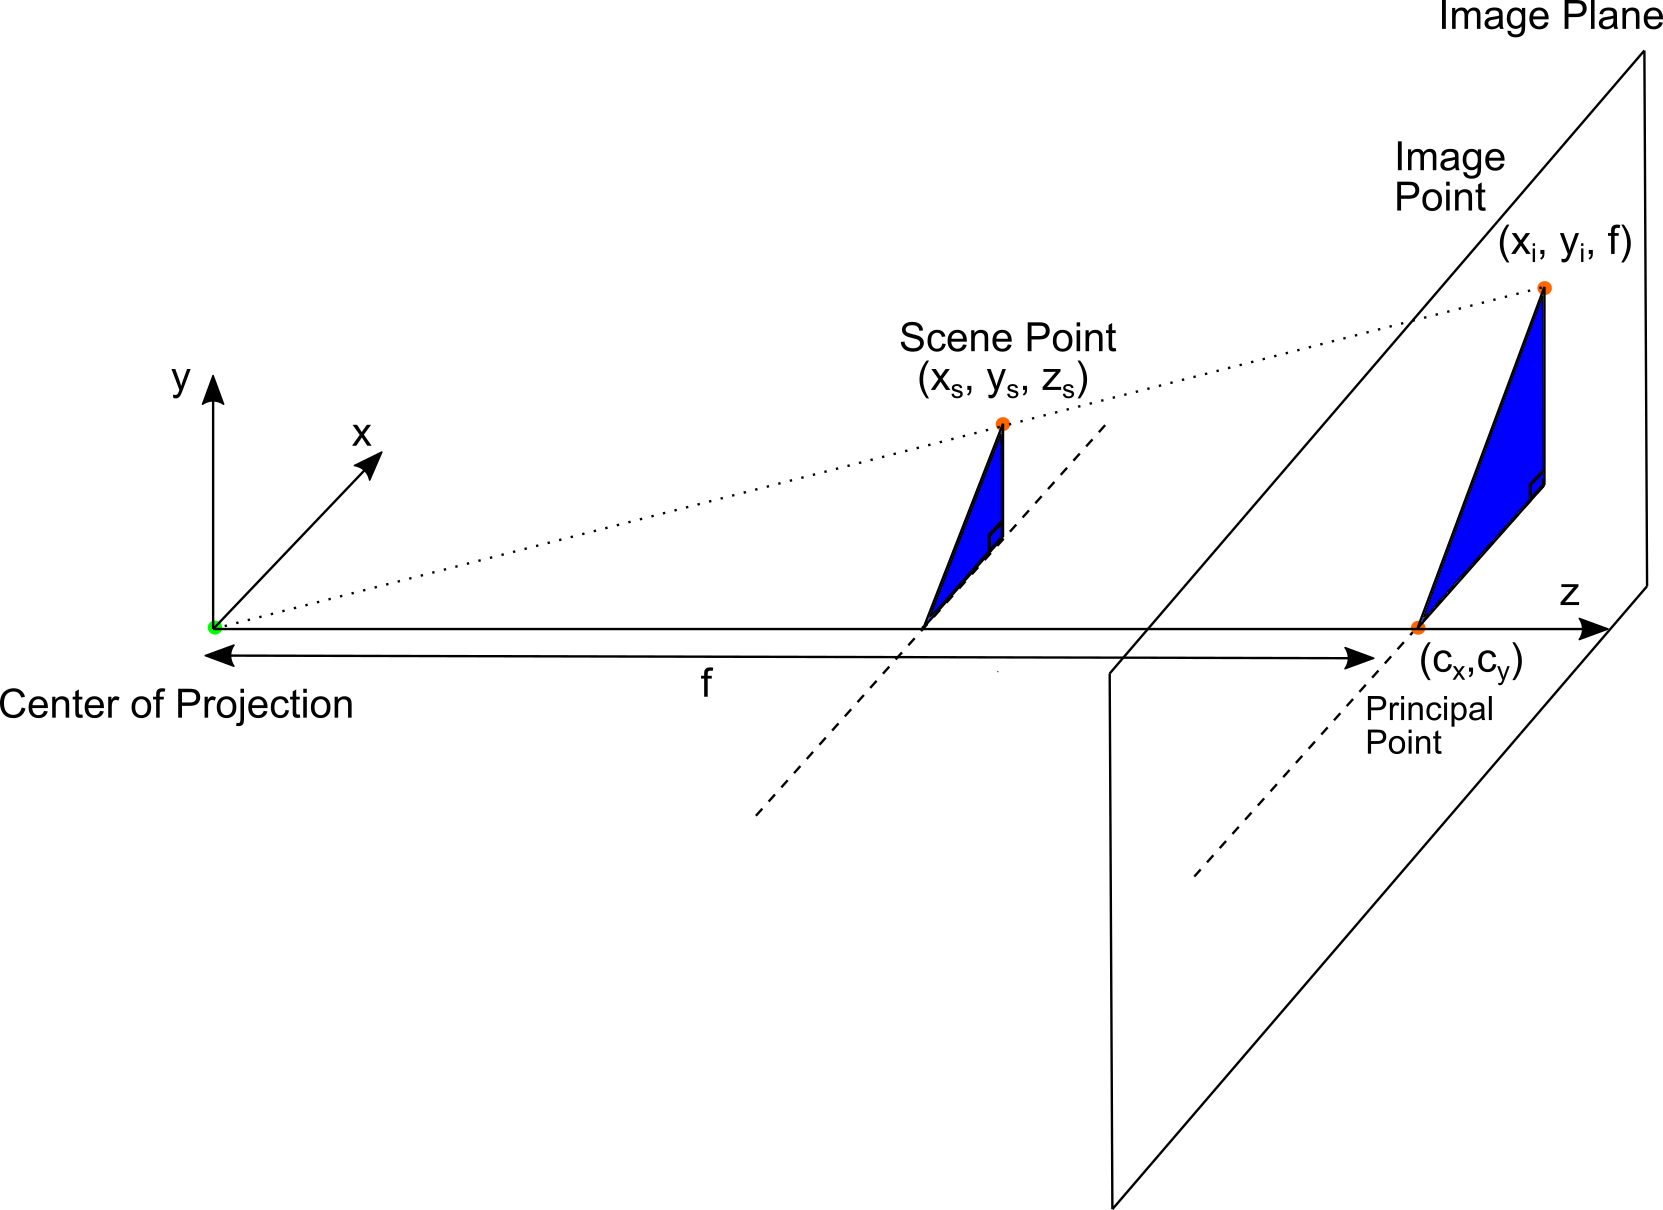
\includegraphics[width=0.85\linewidth]{figs/background/png/perspective-projection.png}
    \end{center}
    \caption{The geometry of perspective projection can be visualized by using similar triangles. The overall scaling of the image is based on the ratio of the focal length to the depth of the object.}
    \label{fig:perspective-projection}
\end{figure}


\begin{equation}
    \begin{aligned}
        \tilde{\mathbf{x}}_{i} &= \begin{bmatrix}
            f' & 0 & 0 \\ 0 & f' & 0 \\ 0 & 0 & 1 
        \end{bmatrix} \tilde{\mathbf{p}}' \\
        &\text{where} \\
        x_i &= p_x'\frac{f'}{p_z'} \\
        y_i &= p_y'\frac{f'}{p_z'} \\
    \end{aligned}
    \label{eq:perspective-projection}
\end{equation}

We can account for any image offset using the principal point. This is the point where the ray from the x-ray to the image plane is perpendicular, which is typically near the center of the image, though not always.

\begin{equation}
    \begin{aligned}
        \tilde{\mathbf{x}}_{i} &= \begin{bmatrix}
            f' & 0 & c_x \\ 0 & f' & c_y \\ 0 & 0 & 1 
        \end{bmatrix} \tilde{\mathbf{p}}' \\
        &\text{where} \\
        c_x &\approx \frac{W_{image}}{2} \\
        c_y &\approx \frac{H_{image}}{2} \\
    \end{aligned}
    \label{eq:perspective-projection}
\end{equation}

Lastly, we need to convert the points in $\tilde{\mathbf{x}}_i$ to pixel coordinates using the pixel scale factor, $k_x,k_y$ for the x and y factors, respectively.

\begin{equation}
    \begin{aligned}
        \tilde{\mathbf{x}}_{pix} &= \begin{bmatrix}
            k_x & 0& 0 \\ 0 & k_y & 0 \\ 0 & 0 & 1
        \end{bmatrix} \begin{bmatrix}
            f' & 0 & c_x \\ 0 & f' & c_y \\ 0 & 0 & 1 
        \end{bmatrix} \\
        & = \begin{bmatrix}
            f_x & 0 & c_x \\ 0 & f_y & c_y \\ 0 & 0 & 1 
        \end{bmatrix}\\
        &\text{where}\\
        f_x &= k_x f' \text{        and        } f_y = k_y f' \\
        &\text{Are focal distances in units of pixels} 
    \end{aligned}
\end{equation}
\subsection{Image Similarity Metrics}
One of the key components in model image registration is image similarity. Fundamentally, this is the method of determining how well the user's synthetic image matches with the actual fluoroscopic image. The choice of similarity metric is going to be determined by many key factors such as the a-priori availability of implant/bone geometry and knowledge of the image quality and contrast. Broadly, there are two classes of image similarity when performing model-image registration: intenisty-based and feature-based.

\subsubsection{Intensity Based}
Intensity based measures are those that utilize specific pixel information in order to determine the difference between two images. This can be either a global image similarity metric, or measure the specfic regions of interest in the given image. 

A canonical difference between two images would be the p-norm separating them (Eq. \ref{eq:p-norm}), which iterates through each pixel of the two images and finds the p-norm difference each intensity for the pixel pair. Common p-norms are the $L_1$ norm (\emph{absolute intensity differences} or \emph{mean absolute difference}) \cite{kanadeStereoMatchingAlgorithm1994} ($p=1$) and the $L_{2}$, or Euclidean, norm (\emph{squared intensity differences} or \emph{mean squared difference}) \cite{hannahComputerMatchingAreas1977}($p=2$).

Intensity-based measures use the pixel values of the images to determine their similarity. These measures can be global, meaning they consider the entire image, or they can focus on specific regions of interest. A common intensity-based measure is the p-norm (Eq. \ref{eq:p-norm}), which calculates the difference between the intensity of corresponding pixels in the two images. The $L_1$ norm, also known as the absolute intensity differences or mean absolute difference, uses $p=1$ in the equation \cite{kanadeStereoMatchingAlgorithm1994}, while the $L_2$ norm, also known as the squared intensity differences or mean squared difference, uses $p=2$ \cite{hannahComputerMatchingAreas1977}. 

\begin{equation}
    \|A-B\|_{p} = (\sum_{x=0}^{w}\sum_{y=0}^{h}|a_{xy}-b_{xy}|^{p})^{\frac{1}{p}}
    \label{eq:p-norm}
\end{equation}

where $A$ and $B$ are the two images being compared, $w$ and $h$ are the width and height of the images, and $a_{xy}$ and $b_{xy}$ are the intensity values at pixel $(x,y)$ in the two images, respectively.

While conceptually easy to use, the main limitation of p-norm measures is their lack of spatial information. For example, an image that has been shifted by a linear transformation would not score well using a p-norm, despite the two images containing only a minor shift, scale, or rotation. One method for overcoming this limitation is to use the cross-correlation, or sliding dot product, between images \cite{bendatRandomDataAnalysis2010,hannahComputerMatchingAreas1977} (Eq. \ref{eq:xcorr}). When used in conjunction with projective geometry, this can help locate regions of interest for a model-based registration pipeline. The cross-correlation is calculated using the following equation:

\begin{equation}
    \begin{aligned}
        (A \star B)[x,y] &= E[A_{xy} \cdot B_{x + \tau_x,y+\tau_y}] \\
        &= \sum_{\tau_x=-\infty}^{\infty}\sum_{\tau_y=-\inf}^{\infty}a_{xy}b_{x + \tau_x,y + \tau_y}
    \end{aligned}
    \label{eq:xcorr}
\end{equation}

This will have the effect of determining the regions of each image that are similar, causing the correlation function to ``light up'' at those areas in a similar way to the convolutional operation between two images. The normalized cross-correlation can also be used (Eq. \ref{eq:norm-xcorr}), which removes noise coming from each of the original images.

\begin{equation}
    \begin{aligned}
        \text{normalized cross correlation}(A,B) &= \frac{A \star B}{(A \star A)(B \star B)}
    \end{aligned}\label{eq:norm-xcorr}
\end{equation}

\subsubsection{Feature Based}
Feature based image similarity metrics involve some method of determining key features in images, and using those notable features for measuring the differences between two images. These types of methods almost always involve some type of feature-extraction step, where the various features of interest are calculated and deterimined for subsequent use. The two main classes of features are \emph{keypoints} and \emph{edges}. The simplest method of keypoint detection is using a similar method to intensity-based matching, but having one of the ``images'' as a patch of the desired feature. With keypoints detected in the input image, one could determine the error of the current pose estimate by taking the Euclidean distance between all image keypoints and all projected keypoints: \cite{burtonAutomaticTrackingHealthy2021} (Eq. \ref{eq:kp-error}). With a-priori information about the keypoints, one could attach a weight to every keypoint in order to emphasize specific regions on the image and the model (Eq. \ref{eq:wkp-error})

\begin{equation}
    \begin{aligned}
        \text{Keypoint Error}= (\sum_{i = 0}^{N}(KP_{image,i} - KP_{proj,i})^2)^{\frac{1}{2}}
    \end{aligned}
    \label{eq:kp-error}
\end{equation}

\begin{equation}
    \begin{aligned}
        \text{Weighted Keypoint Error} = (\sum_{i = 0}^{N}w_{i}(KP_{image,i} - KP_{proj,i})^2)^{\frac{1}{2}}
    \end{aligned}
    \label{eq:wkp-error}
\end{equation}

Keypoints are particularly useful when there are invariant features in images and 3D models that will always be present. However, if these features will not, or cannot always be deteted, then other measures must be utilized.

\emph{Finding Edges}\\
Edge- and contour-based matching algorithms make use of the edges that are present in the image, and aligning that with a the projected edges of the 3D model. However, we must first consider the determination of edges in an images. For a human operator, it can be rather easy to find edges of interest, but how much this be incorporated computationally? The first approach might be in viewing an image topologically, with regions of different colors and intensity represented by different ``heights''. Then, an edge simply becomes an area with a steep gradient (Eq. \ref{eq:img-grad}).

\begin{equation}
    \begin{aligned}
        \mathbf{J}(\mathbf{x}) = \nabla I(\mathbf{x}) = (\frac{\partial I}{\partial x}, \frac{\partial I}{\partial y})(\mathbf{x})
    \end{aligned}
    \label{eq:img-grad}
\end{equation}

Finding the direction of the steepest ascent/descent at any given location will give use the normal to the local edge at that point. However, the derivative operator will accentuate and amplify high frequencies in the image, causing noise to overpower the signal. Removing the high-frequency information (a low-pass filter) in the image results in gradient detection that is much more aligned with the salient edges of the image. The Gaussian kernel is a good option for an isotropic low-pass filter on a 2D signal (image) (Eq. \ref{eq:gauss-kernel-grad})

\begin{equation}
    \begin{aligned}
        \mathbf{J}_{\sigma}(\mathbf{x}) &= \nabla [G_\sigma (\mathbf{x} * I(\mathbf{x}))] \\
        &= \nabla G_\sigma (\mathbf{x}) * I(\mathbf{x}) \\
        &\text{where} \\
        \nabla G_\sigma (\mathbf{x}) &= (\frac{\partial G_{\sigma}}{\partial x}, \frac{\partial G_{\sigma}}{\partial x}) = [-x - y]\frac{1}{\sigma^{2}}\text{exp}(\frac{-(x^2 + y^2)}{2 \sigma^2})
    \end{aligned}
    \label{eq:gauss-kernel-grad}
\end{equation}


The ubiquitous edge detection algorithm was proposed by John Canny in 1986 \cite{cannyComputationalApproachEdge1986}, which utilizes a five-step process. First, a Gaussian kernel is applied as a low-pass filter (Eq. \ref{eq:gauss-kernel-grad}), second, directional filters are used to find the gradients in each direction of the image, third, a gradient magnitude threshold is applied to remove noise, fourth, a double threshold is applied to remove both strong and weak edges, and lastly, edges are determined from hysteresis. 

\emph{Using Edges for Image Similarity}\\
In model-image registration, the similarity of two contours is used as a heuristic for the correct pose. When the projected model's contour aligns accurately with the edges in the fluoroscopic image, one can say that the model is \emph{properly registered} to the image. The main question becomes: how can we computationally determine when two contours are aligned?

As always, the simplest approach is to take the p-norm between the model and image contours (Eq. \ref{eq:p-norm}), where instead of taking the difference between the two original images, one is taking the difference of the edges of the images. This function will be minimized when there is complete overlap between image and model contours. The primary issue with this formulation is the sensitivity to slight perturbations in the model. This is due to the width of the contour being a single pixel, which would render an extremely high error if the model is shifted just a single pixel in any direction. Because the edge-detected images are binary (0-no edge, 1-edge), we can take advantage of binary morphological operations to change the images to better suit the model-image registration pipeline. The primary operation is dilation (Eq. \ref{eq:dilation}), which is simply the convolutional operation with the kernel containing all 1s.

\begin{equation}
\begin{aligned}
    I_{dil} &= (I \circledast g)\\
    &\text{where} \\
    g &= \begin{pmatrix}
        1 & 1 & 1 \\ 1 & 1 & 1 \\ 1& 1 & 1
    \end{pmatrix}
\end{aligned}
\label{eq:dilation}
\end{equation}

The dilation operator is useful because it decreases the sensitivity of the p-norm metric for image similarity, allowing for a smoother curve for optimization routines to find a global minima.

\subsubsection{Symmetry Traps}
Objects with rotational or mirror symmetry cause pathological solutions to many of the image similarity metrics when used for optimizing the pose of the object relative to the image. The simplest example of a symmetry trap can be posed as follows: given the shadow of a basketball, which direction was the logo facing? It is quickly apparent that this is an impossible question to answer with just the information given by the image and the 3D model. This problem arises when performing optimizing for the post of mediolaterally symmetric tibial implants. Additional information must be used to find the correct pose of the implant.

However, with the knowledge of the direction of symmetry, it is possible to determine the ``dual pose'' of the current orientation, that is, the pose that produces indistinguishable projective geometry.

\begin{mdframed}
    \begin{center}
        {\bf Algorithm for Determining the Dual-Pose of a Symmetric Object}
    \end{center}
\begin{enumerate}
    \item Determine the viewing ray from camera $\rightarrow$ object (Eq. \ref{eq:view-ray}).
    \item Determine the axis-angle ($m,\theta$) rotation between the viewing ray and the symmetric axis of the object (Eq. \ref{eq:angle-between}, \ref{eq:perp-axis}).
    \item Rotate the object $-2\theta$ about the same axis, reflecting the rotation about the viewing ray (Eq. \ref{eq:equiv-axs-angle}).
    \item The final orientation of the object is exactly the ``dual pose'', producing indistinguishable projective geometry (Eq. \ref{eq:rotation-matrix-mult}).
\end{enumerate}
\end{mdframed}

\begin{equation}
    \begin{aligned}
        \text{If $T$ is the homogenous}& \text{ transformation matrix describing the object} \\
        \vec{v}' &= T_{1:3,4} \\
        \vec{v} & = \frac{\vec{v}'}{\|\vec{v}'\|}
    \end{aligned}
    \label{eq:view-ray}
\end{equation}


We can use trigonometry to determine the angle (Eq. \ref{eq:angle-between}) and perpindicular axis (Eq. \ref{eq:perp-axis}) between two vectors. For our example, we use the normalized viewing ray and the z-axis (symmetric axis) as the two vectors.
\begin{equation}
    \begin{aligned}
        cos(\theta) &= \vec{v} \cdot \vec{z} \\
        &\rightarrow \\
        \theta &= arccos(\vec{v} \cdot \vec{z})
    \end{aligned}
    \label{eq:angle-between}
\end{equation}

\begin{equation}
    \begin{aligned}
        \vec{m} = \frac{\vec{v} \times \vec{z}}{\|\vec{v} \times \vec{z}\|}
    \end{aligned}
    \label{eq:perp-axis}
\end{equation}

Then, we can build a rotation matrix using an axis and an angle \cite{craneKinematicAnalysisRobot2008}, (Eq. \ref{eq:equiv-axis-angle}).

\begin{equation}
    \begin{aligned}
        c &= cos(-2\theta)\\
        s &= sin(-2\theta) \\
        q &= -cos(-2\theta)\\
        R_{3 \times 3} &= \begin{pmatrix}
            m_x^2v + c & m_xm_yv - m_zs & m_x m_z v - m_y s \\ m_x m_y v + m_z s & m_y^2 v + c & m_y m_z v - m_x s \\ m_x m_z v - m_y s & m_y m_z v + m_x s & m_z^2 v + c
        \end{pmatrix}
    \end{aligned}
    \label{eq:equiv-axis-angle}
\end{equation}

Then, we obtain the final transformation matrix describing the dual pose of the object by a post-multiplication of this rotation matrix.

\begin{equation}
    \begin{aligned}
        T_{dual} = T_{orig} * \begin{pmatrix}
            R_{3 \times 3} & \vec{0}_{3 \times 1} \\ \vec{0}_{1 \times 3} & 1
        \end{pmatrix}
    \end{aligned}
    \label{eq:rotation-matrix-mult}
\end{equation}

Given these two matrices, further exploration can determine which is the correct pose, though this will have to be done using information not directly present in the image contours.